%!TeX program = xelatex
%Do not change
\documentclass[12pt, oneside]{article}
\usepackage{amssymb,amsmath}
\usepackage[margin=1in]{geometry}
\usepackage{textpos}
\usepackage{float}
\usepackage{booktabs}
%\usepackage{color}
\usepackage{graphicx}
\usepackage[inter-unit-product =\cdot]{siunitx}
\let\DeclareUSUnit\DeclareSIUnit
\let\US\SI
\DeclareUSUnit\inch{in}
\DeclareUSUnit\foot{ft}
\DeclareUSUnit\mile{mi}
\DeclareUSUnit\foot{ft}
\DeclareUSUnit\slug{slug}
\DeclareUSUnit\pound{lb}
\DeclareUSUnit\psi{psi}
\DeclareUSUnit\Msi{Msi}
\DeclareUSUnit\ksi{ksi}

%\usepackage{tikz}
%\usetikzlibrary{positioning}
%\usepackage{tikz-3dplot}
%\usepackage{pgfopts}
%\usepackage{wasysym}
%\usepackage{stanli}

% You may add the packages you need here
\begin{document}

%TODO change numbers in problems
\begin{textblock*}{4cm}(-1.7cm,-2.3cm)
\noindent {\scriptsize AE333 Fall 2021}
\end{textblock*}

%Do not modify other than putting your name where stated
\begin{textblock*}{8cm}(12.5cm,-1cm)
\noindent {Name: }
\end{textblock*}
%Do not modify other than typing your acknowledgement where stated
\begin{textblock*}{13.5cm}(-1.7cm,-1.8cm)
%\noindent \textit{\footnotesize Acknowledgement: Your acknowledgement for collaboration and other sources goes here. }
\end{textblock*}

\vspace{1cm}

%Do not modify other than typing the homework number after #
\begin{center}
\textbf{\Large Homework 9}

\textbf{Due 19 November 2021}
\end{center}

\begin{enumerate}
	\item %12-6
		Find the deflection (as a function of $x$) for a cantilevered beam with an applied end moment.
		Assume $EI$ is constant and express answer in terms of applied moment and $EI$.
		\begin{figure}[H]
			\centering
			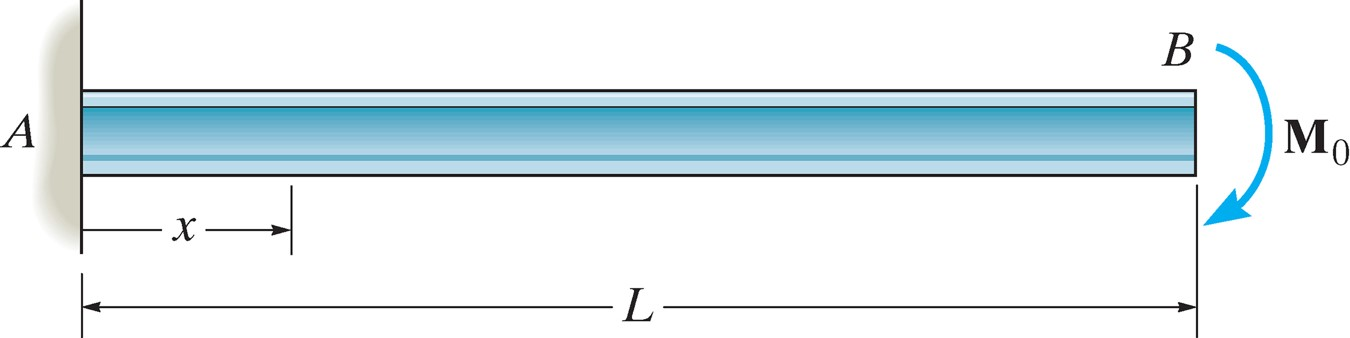
\includegraphics[width=0.6\linewidth]{12-6}
		\end{figure}

	\item %12-15
		A torque wrench is used to tighten the nut on a bolt.
		If the dial indicates that a torque of $ 	\US{75}{ft.lb}  $ when the bolt is fully tightened, find the force $P$ on the handle and the distance that the needle moves along the scale.
		Assume that only the section $AB$ bends and the cross section is a solid $ 	\US{0.5 }{in}  $ square with $E = 	\US{29 }{Msi} $
		\begin{figure}[H]
			\centering
			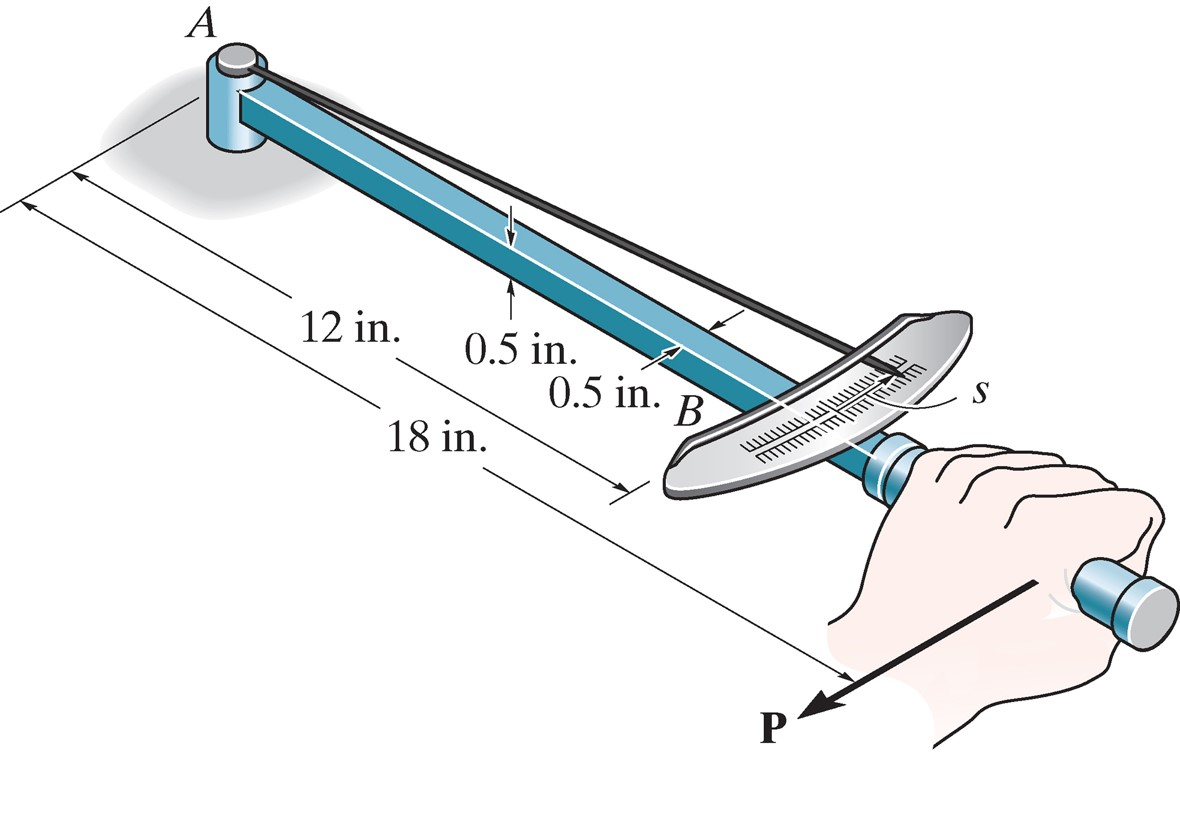
\includegraphics[width=0.6\linewidth]{12-15}
		\end{figure}
		\newpage

	\item %12-25
		The floor beam of an airplane is subjected to the loading shown.
		Assuming the fuselage exerts only vertical reactions on the ends of the beam, determine the maximum deflection of the beam in terms of some constant flexural rigidity, $EI$.
		\begin{figure}[H]
			\centering
			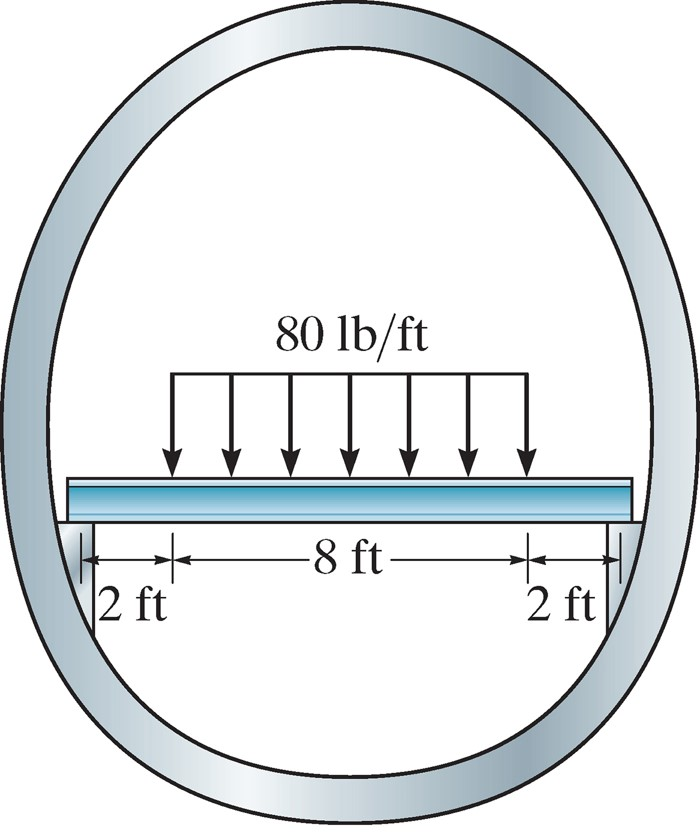
\includegraphics[width=0.6\linewidth]{12-25}
		\end{figure}

	\item %12-35
		Find the deflection as a function of $x$ for the beam shown in terms of some constant $EI$.
		\begin{figure}[H]
			\centering
			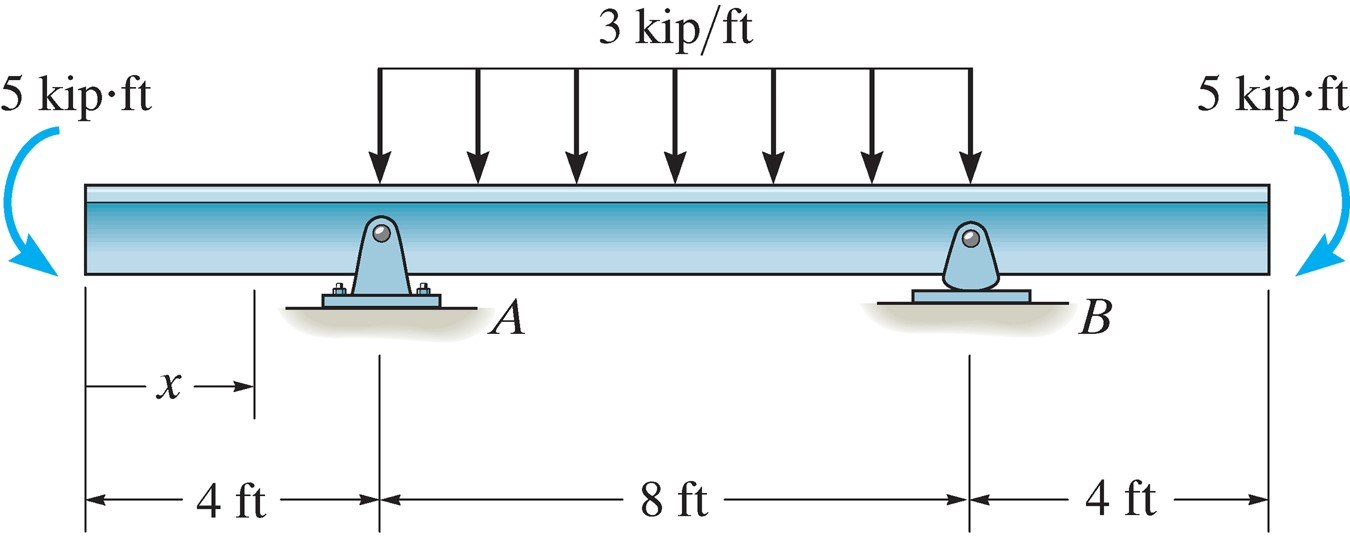
\includegraphics[width=0.6\linewidth]{12-35}
		\end{figure}
		\newpage

	\item %12-39
		Find the deflection as a function of $x$ for the beam shown in terms of some constant $EI$.
		\begin{figure}[H]
			\centering
			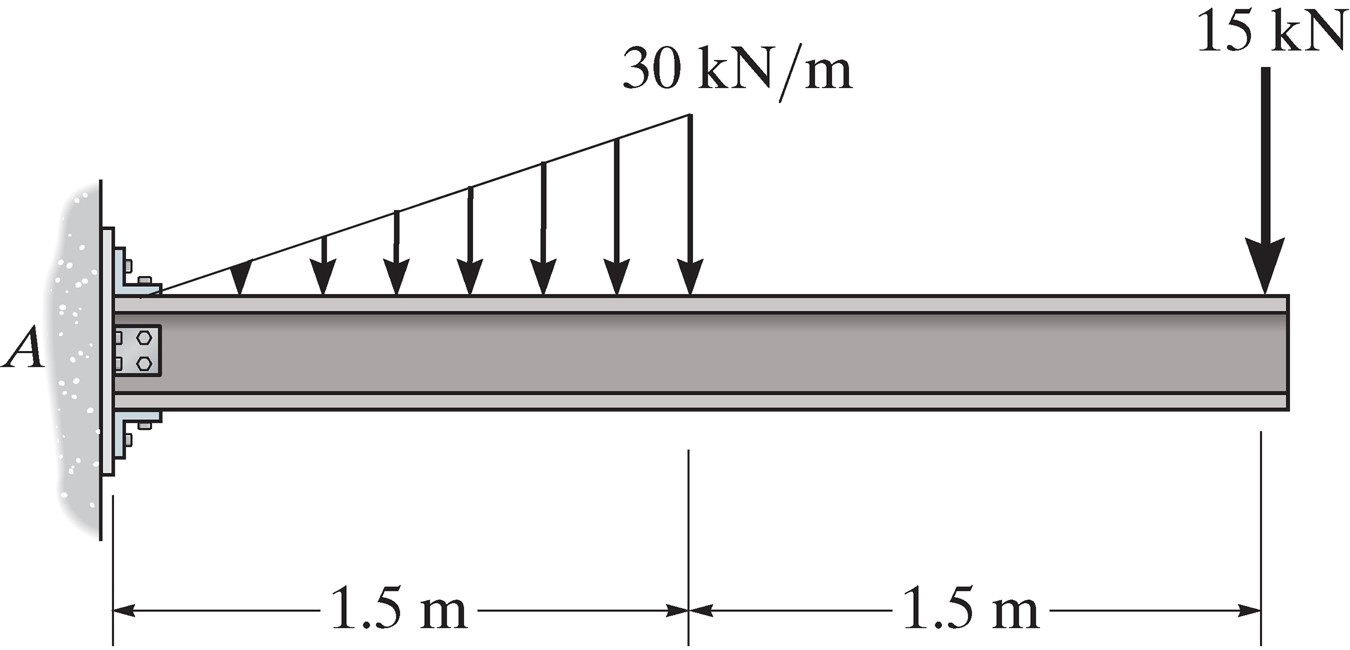
\includegraphics[width=0.6\linewidth]{12-39}
		\end{figure}

	\item %12-93
		The rod is pinned at the end $A$ and attached to a torsional spring with stiffness $k$ (with $k$ expressed in torque per radian of rotation).
		For a perpendicular force, $P$, as shown find the displacement of the force in terms of some constant $EI$.
		\begin{figure}[H]
			\centering
			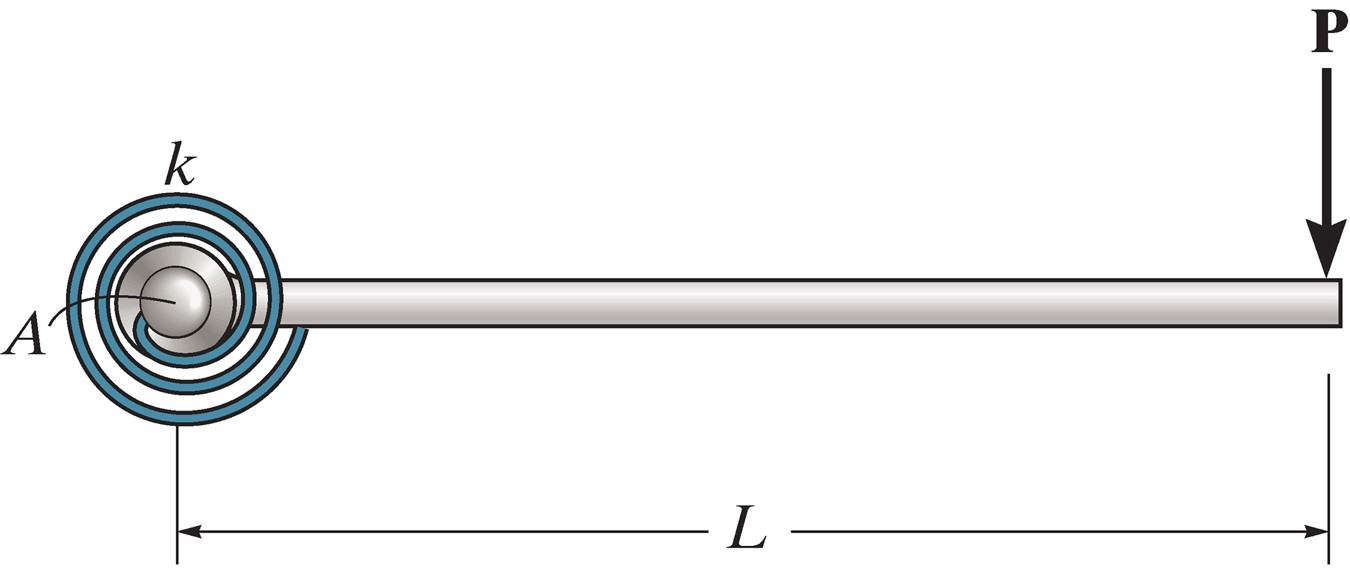
\includegraphics[width=0.6\linewidth]{12-93}
		\end{figure}

\end{enumerate}
\end{document}
